\documentclass[border=10mm]{standalone}
\usepackage{tikz}
\usepackage{amsmath}
\usepackage{amssymb}
\usepackage{bm}
\usetikzlibrary{arrows.meta, fit, backgrounds, calc}

%%─── Palette ────────────────────────────────────────────────────────────────
\definecolor{tBlue}    {RGB}{52,119,196}
\definecolor{sGreen}   {RGB}{56,142,60}
\definecolor{mlmOrange}{RGB}{230,130,30}
\definecolor{lossRed}  {RGB}{198,40,40}
\definecolor{pPurple}  {RGB}{123,31,162}
\definecolor{eGold}    {RGB}{180,140,0}

%%─── Node styles ────────────────────────────────────────────────────────────
\tikzset{
  nd/.style   = {draw, rounded corners=5pt, align=center, inner sep=7pt,
                 minimum width=4.0cm, minimum height=0.9cm, font=\small},
  T/.style    = {nd, draw=tBlue,    fill=tBlue!10},
  S/.style    = {nd, draw=sGreen,   fill=sGreen!10},
  ENC/.style  = {nd, draw=eGold,    fill=eGold!15},
  MLM/.style  = {nd, draw=mlmOrange,fill=mlmOrange!18},
  PL/.style   = {nd, draw=pPurple,  fill=pPurple!12},
  LO/.style   = {nd, draw=lossRed,  fill=lossRed!10, minimum width=3.6cm},
  %% Arrows
  Tarr/.style ={-{Stealth[length=5pt]}, thick, tBlue!60, dashed},
  Sarr/.style ={-{Stealth[length=5pt]}, thick, sGreen!70},
  Larr/.style ={-{Stealth[length=4pt]}, thick, lossRed},
}

%% ─── Column x-centres ───────────────────────────────────────────────────────
%%  Teacher (stop-grad, full doc) : x =  0
%%  Student (para-pred kept doc)  : x =  8
%%  MLM    (token-masked doc)     : x = 16
%%  L_para_pred (between T and S) : x =  4
%%  L_mlm  (directly under MLM)   : x = 16, y = -12.5
%%  L_total                       : x =  8, y = -15.5

%% ─── Row y-positions (cm, downward = more negative) ─────────────────────────
%%  Input        : y =   0
%%  Encoder      : y =  -2.5
%%  Hidden / CLS : y =  -5.0
%%  Pool / Head  : y =  -7.5
%%  Output repr  : y = -10.0

\begin{document}
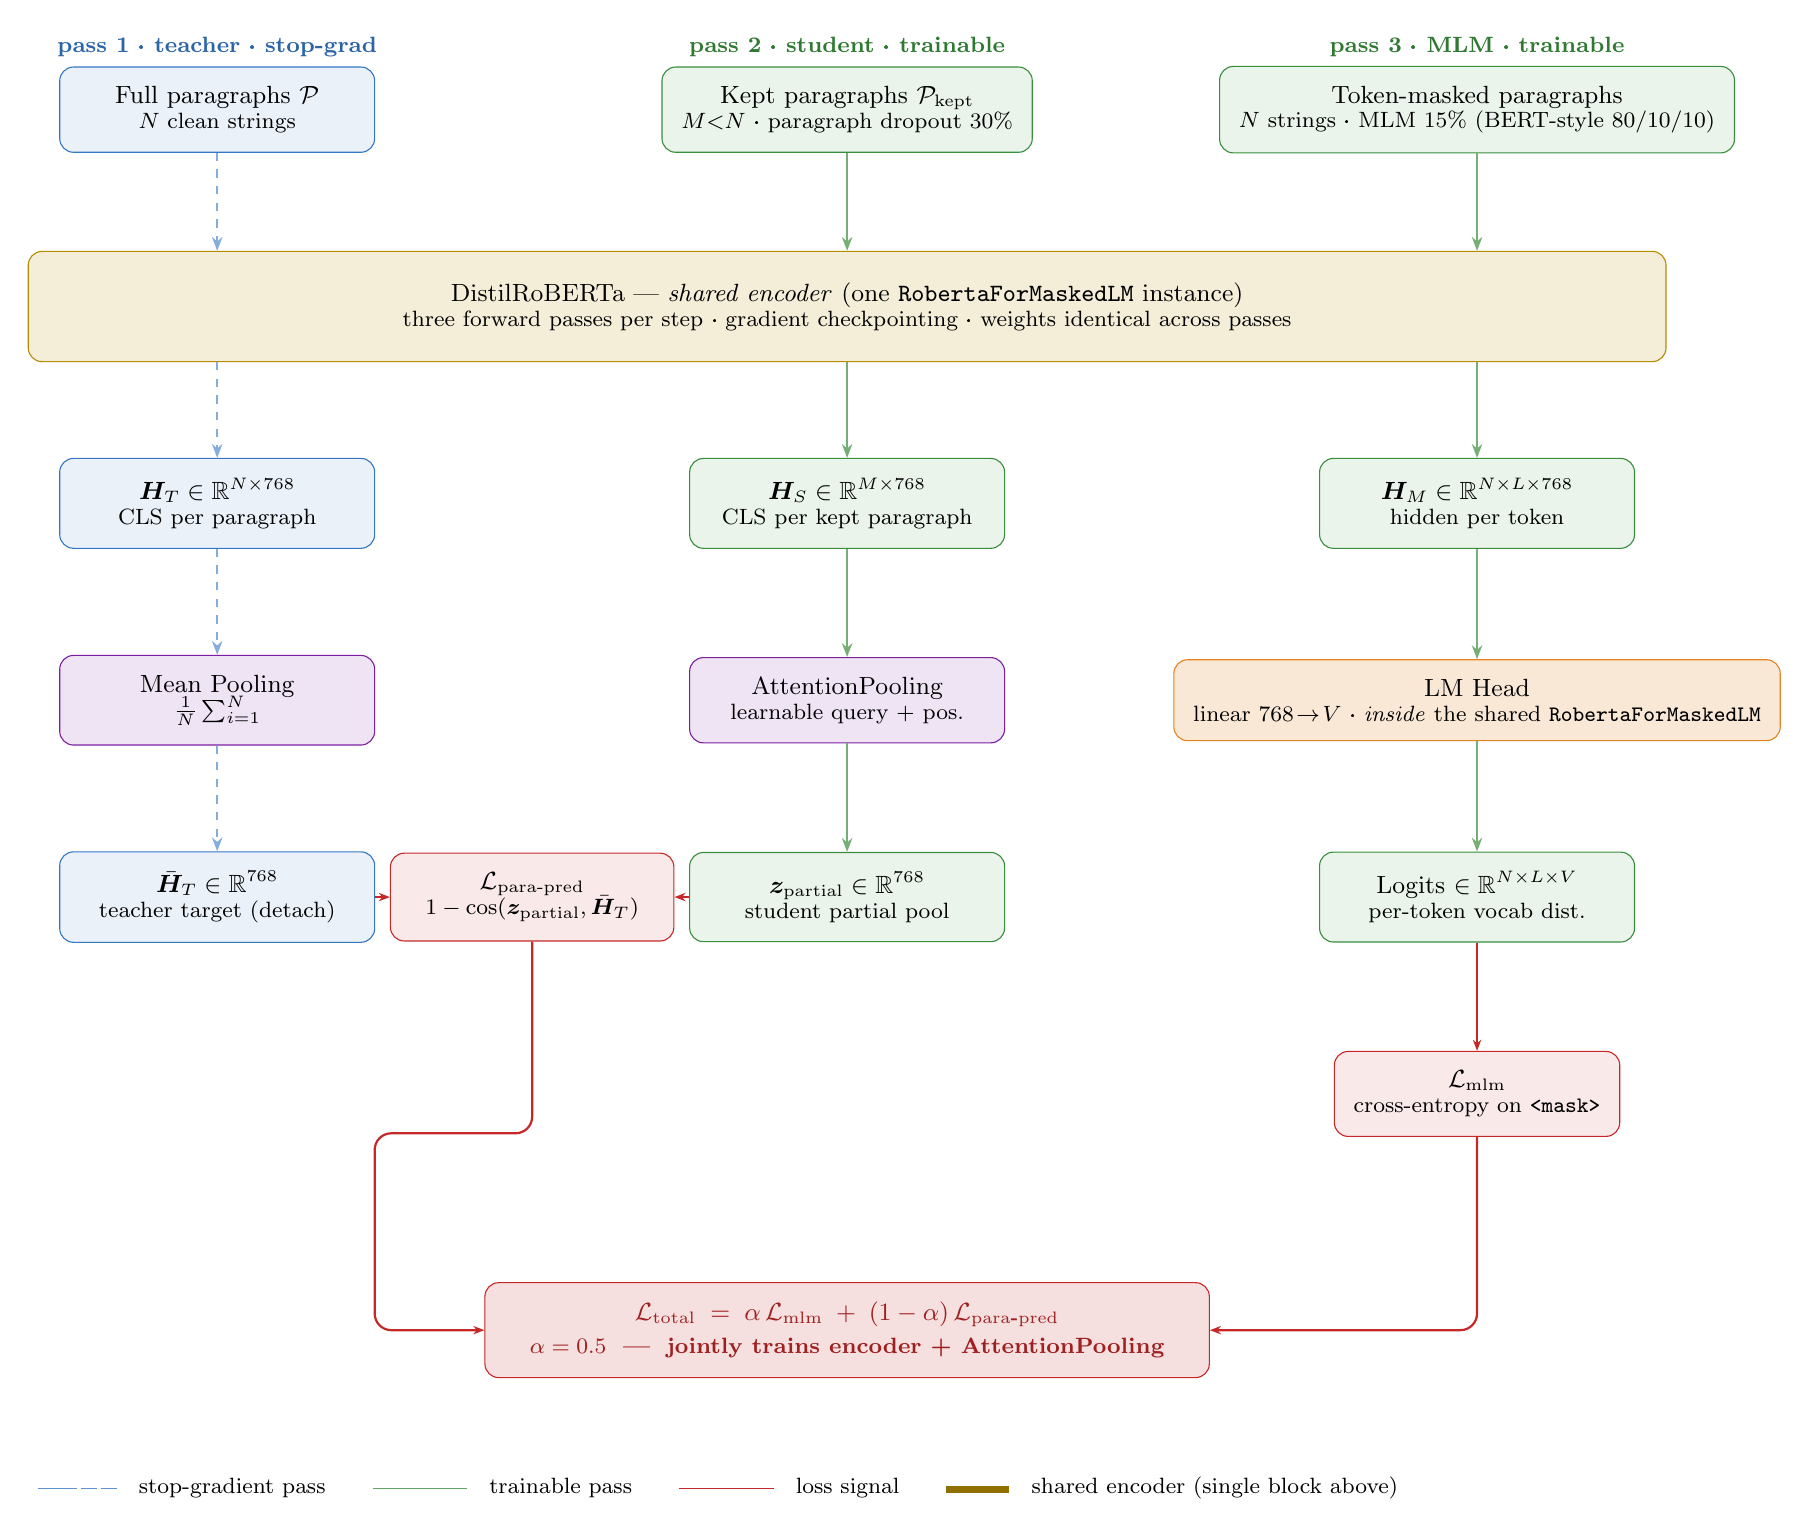
\begin{tikzpicture}

%% ═══════════════════════════════════════════════════════
%%  SHARED ENCODER — one RobertaForMaskedLM, three passes
%% ═══════════════════════════════════════════════════════
\node[ENC, minimum width=20.8cm, minimum height=1.4cm]
     (enc) at ( 8, -2.5) {DistilRoBERTa --- \emph{shared encoder} (one \texttt{RobertaForMaskedLM} instance)\\[-2pt]
                          \footnotesize three forward passes per step · gradient checkpointing · weights identical across passes};


%% ═══════════════════════════════════════════════════════
%%  TEACHER track — stop-gradient pass, full document (x = 0)
%% ═══════════════════════════════════════════════════════

\node[T]   (t_in)  at ( 0,   0  ) {Full paragraphs $\mathcal{P}$\\[-2pt]
                                    \footnotesize $N$ clean strings};

\node[T]   (t_cls) at ( 0,  -5.0) {$\bm{H}_T\in\mathbb{R}^{N\times768}$\\[-2pt]
                                    \footnotesize CLS per paragraph};

\node[PL]  (t_mp)  at ( 0,  -7.5) {Mean Pooling\\[-2pt]
                                    \footnotesize $\frac{1}{N}\sum_{i=1}^{N}$};

\node[T]   (t_tg)  at ( 0, -10.0) {$\bar{\bm{H}}_T\in\mathbb{R}^{768}$\\[-2pt]
                                    \footnotesize teacher target (detach)};

\draw[Tarr] (t_in.south)               -- (enc.north -| t_in.south);
\draw[Tarr] (enc.south -| t_cls.north) -- (t_cls.north);
\draw[Tarr] (t_cls)--(t_mp);
\draw[Tarr] (t_mp) --(t_tg);


%% ═══════════════════════════════════════════════════════
%%  STUDENT track — trainable pass, paragraph-dropout (x = 8)
%% ═══════════════════════════════════════════════════════

\node[S]   (s_in)  at ( 8,   0  ) {Kept paragraphs $\mathcal{P}_{\mathrm{kept}}$\\[-2pt]
                                    \footnotesize $M{<}N$ · paragraph dropout $30\%$};

\node[S]   (s_cls) at ( 8,  -5.0) {$\bm{H}_S\in\mathbb{R}^{M\times768}$\\[-2pt]
                                    \footnotesize CLS per kept paragraph};

\node[PL]  (s_pl)  at ( 8,  -7.5) {AttentionPooling\\[-2pt]
                                    \footnotesize learnable query + pos.};

\node[S]   (s_zp)  at ( 8, -10.0) {$\bm{z}_{\mathrm{partial}}\in\mathbb{R}^{768}$\\[-2pt]
                                    \footnotesize student partial pool};

\draw[Sarr] (s_in.south)               -- (enc.north -| s_in.south);
\draw[Sarr] (enc.south -| s_cls.north) -- (s_cls.north);
\draw[Sarr] (s_cls)--(s_pl);
\draw[Sarr] (s_pl) --(s_zp);


%% ═══════════════════════════════════════════════════════
%%  MLM track — trainable pass, token-masked (x = 16)
%% ═══════════════════════════════════════════════════════

\node[S]   (m_in)  at (16,   0  ) {Token-masked paragraphs\\[-2pt]
                                    \footnotesize $N$ strings · MLM $15\%$ (BERT-style $80/10/10$)};

\node[S]   (m_hs)  at (16,  -5.0) {$\bm{H}_M\in\mathbb{R}^{N\times L\times768}$\\[-2pt]
                                    \footnotesize hidden per token};

\node[MLM] (m_lm)  at (16,  -7.5) {LM Head\\[-2pt]
                                    \footnotesize linear $768\!\to\!V$ · \emph{inside} the shared \texttt{RobertaForMaskedLM}};

\node[S]   (m_lg)  at (16, -10.0) {Logits $\in\mathbb{R}^{N\times L\times V}$\\[-2pt]
                                    \footnotesize per-token vocab dist.};

\draw[Sarr] (m_in.south)              -- (enc.north -| m_in.south);
\draw[Sarr] (enc.south -| m_hs.north) -- (m_hs.north);
\draw[Sarr] (m_hs)--(m_lm);
\draw[Sarr] (m_lm) --(m_lg);


%% ═══════════════════════════════════════════════════════
%%  LOSS NODES
%% ═══════════════════════════════════════════════════════

%% L_para_pred — cosine, partial vs full-doc target
\node[LO] (l_pp) at ( 4, -10.0) {$\mathcal{L}_{\mathrm{para\text{-}pred}}$\\[-2pt]
                                   \footnotesize $1 - \cos(\bm{z}_{\mathrm{partial}},
                                                          \bar{\bm{H}}_T)$};
\draw[Larr] (t_tg.east)--(l_pp.west);
\draw[Larr] (s_zp.west)--(l_pp.east);

%% L_mlm — token-level cross-entropy
\node[LO] (l_mlm) at (16, -12.5) {$\mathcal{L}_{\mathrm{mlm}}$\\[-2pt]
                                    \footnotesize cross-entropy on \texttt{<mask>}};
\draw[Larr] (m_lg)--(l_mlm);

%% L_total — combined
\node[LO, minimum width=9.2cm, draw=lossRed,
      fill=lossRed!15, text=lossRed!80!black, font=\small\bfseries]
      (l_tot) at ( 8, -15.5) {%
      $\mathcal{L}_{\mathrm{total}}
       \;=\; \alpha\,\mathcal{L}_{\mathrm{mlm}}
            \;+\;(1-\alpha)\,\mathcal{L}_{\mathrm{para\text{-}pred}}$\\[1pt]
       \footnotesize $\alpha = 0.5$ \;|\; jointly trains encoder + AttentionPooling};

\draw[Larr, rounded corners=6pt]
     (l_pp.south)  -- (4,-13) -- (2,-13) -- (2,-15.5) -- (l_tot.west);
\draw[Larr, rounded corners=6pt]
     (l_mlm.south) -- (16,-15.5) -- (l_tot.east);


%% ═══════════════════════════════════════════════════════
%%  PASS HEADERS — three passes through the SAME encoder
%%  (no colored backgrounds: there is no teacher/student split,
%%   just one model invoked three times per step)
%% ═══════════════════════════════════════════════════════
\node[font=\footnotesize\bfseries, text=tBlue!85!black,  anchor=south]
     at ( 0, 0.55) {pass 1 · teacher · stop-grad};
\node[font=\footnotesize\bfseries, text=sGreen!85!black, anchor=south]
     at ( 8, 0.55) {pass 2 · student · trainable};
\node[font=\footnotesize\bfseries, text=sGreen!85!black, anchor=south]
     at (16, 0.55) {pass 3 · MLM · trainable};


%% ═══════════════════════════════════════════════════════
%%  LEGEND
%% ═══════════════════════════════════════════════════════
\node[font=\footnotesize, anchor=west, align=left]
     at (-2.4,-17.5) {%
  \textcolor{tBlue!80}{\rule[0.4ex]{0.5cm}{0.5pt}%
  \,\rule[0.4ex]{0.2cm}{0.5pt}\,\rule[0.4ex]{0.2cm}{0.5pt}}
  \; stop-gradient pass\qquad
  \textcolor{sGreen!80}{\rule[0.4ex]{1.2cm}{0.5pt}}
  \; trainable pass\qquad
  \textcolor{lossRed}{\rule[0.4ex]{1.2cm}{0.5pt}}
  \; loss signal\qquad
  \textcolor{eGold!80!black}{\rule[0ex]{0.8cm}{2.5pt}}
  \; shared encoder (single block above)
};

\end{tikzpicture}
\end{document}
